The following chapter is dedicated to evaluate the different machine learning and feature engineering methods on
the target compounds. For each protein the top two approaches are evaluated further.

\subsection{Acetylcholinesterase}
The following table presents the results of the different machine learning algorithms on the various
test-sets. The ROC curves for the top two performing configurations can be found at \ref{fig:ache_baseline_rf_roc} and \ref{fig:ache_smote_rf_roc}
respectively. The confusion matrices can be found at \ref{fig:ache_baseline_rf_conf} and \ref{fig:ache_smote_rf_conf}.
The scoring functions achieved a score of 81.06\% on the test-set. 
\begin{table}[H]
    \begin{center}
        \caption{Acetylcholinesterase performance test-set}
        \begin{tabular}{lrrrrr}
            \toprule
            Name             & ACC    & FPR    & AUC    & EF     & REF     \\
            \midrule
            baseline\_rf     & 0.8106 & 0.3285 & 0.7992 & 1.4161 & 92.6829 \\
            fe\_smote\_rf    & 0.8007 & 0.3358 & 0.7894 & 1.4046 & 91.4634 \\
            fe\_smote\_nn    & 0.7708 & 0.2993 & 0.7650 & 1.4102 & 82.9268 \\
            baseline\_nn     & 0.7674 & 0.2920 & 0.7626 & 1.4134 & 81.7073 \\
            fe\_rf\_per\_knn & 0.7575 & 0.4307 & 0.7420 & 1.3172 & 91.4634 \\
            baseline\_knn    & 0.6844 & 0.5766 & 0.6629 & 1.1966 & 90.2439 \\
            fe\_rf\_mdi\_knn & 0.5515 & 0.4307 & 0.5530 & 1.0987 & 59.8639 \\
            \bottomrule
        \end{tabular}
    \end{center}
\end{table}

\begin{figure}[H]
    \begin{center}
        \caption[]{Baseline random forest confusion matrix}
        \label{fig:ache_baseline_rf_conf}
        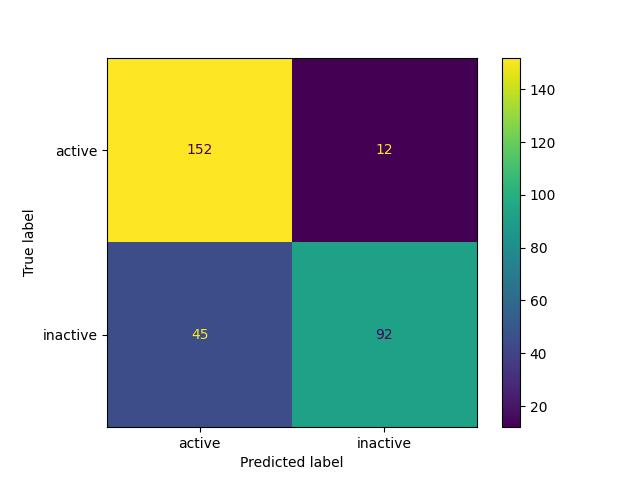
\includegraphics[height=9cm]{ache/baseline_rf_conf.jpg}
    \end{center}
\end{figure}

\begin{figure}[H]
    \begin{center}
        \caption[]{SMOTE random forest confusion matrix}
        \label{fig:ache_smote_rf_conf}
        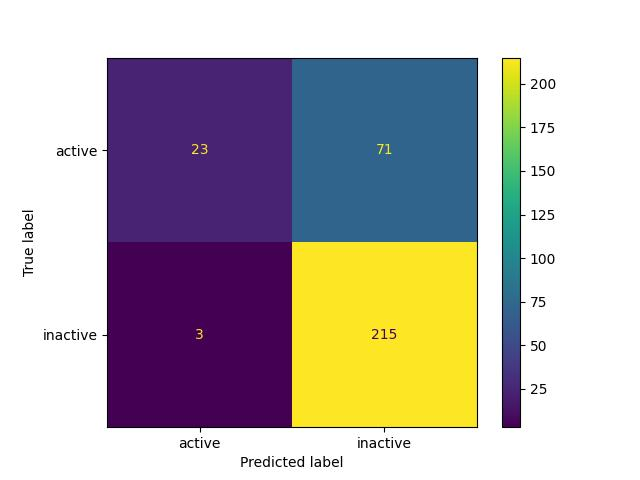
\includegraphics[height=9cm]{ache/fe_smote_rf_conf.jpg}
    \end{center}

\end{figure}

\begin{figure}[H]
    \begin{center}
        \caption[]{Baseline random forest ROC curve}
        \label{fig:ache_baseline_rf_roc}
        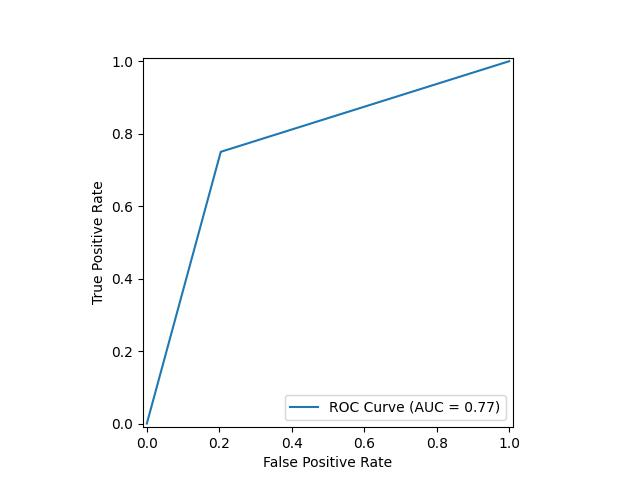
\includegraphics[height=9cm]{ache/baseline_rf_roc.jpg}
    \end{center}

\end{figure}

\begin{figure}[H]
    \begin{center}
        \caption[]{SMOTE random forest ROC curve}
        \label{fig:ache_smote_rf_roc}
        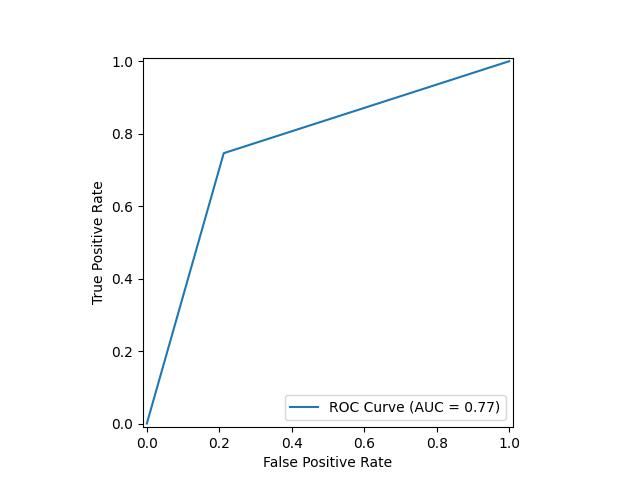
\includegraphics[height=9cm]{ache/fe_smote_rf_roc.jpg}
    \end{center}
\end{figure}


\subsection{Cyclooxygenase 1}

\subsection{Dipeptidyl peptidase IV}
\subsection{Monoamine oxidase B}
\subsection{Soluble epoxide hydrolase}